\section{Styrhandske}
\begin{figure}[H]
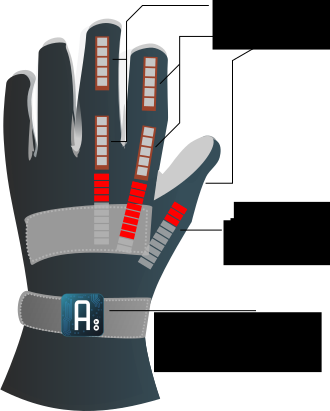
\includegraphics[height=0.5\textheight]{img/kontrollhandske}
\caption{Konceptskiss över styrhandsken.}
\label{kontrollhandske}
\end{figure}
%Detta är intro. Det ska inte vara några detaljer här, bara översiktligt!
% Konvention: styrhandske, inte reglerhandske eller kontrollhanske

För att intuitivt reglera robothanden används en tunn handske som användaren bär på sin hand. På handskens tumme, långfinger och pekfinger finns det två flexsensorer vardera, se figur \ref{kontrollhandske}, som följer användarens hand och ändrar resistans beroende på hur mycket de böjs. På handsken sitter det även tre ledramper som indikerar hur hårt man påverkar objektet. Det tänds fler ledlampor ju större trycket på trycksensorerna är. \comment{borttaget: Resistansen samplas av en mikrokontroller, som efter filtrering trådlöst sänder styrsignaler till robothanden.
Robothanden sänder i sin tur trycket från dess fingrar till styrhandsken. Trycket återkopplas till användaren genom att fler ledlampor på handen tänds ju större trycket är.}


\comment{Emil: Skriv om handens fysiska konstruktion}

\comment{öjeling: fin bild hur signaler åker runt}

\comment{Kanske något enkelet schema för hur det är uppkopplat}




\section{Algoritmer}
Här presenteras de styralgortimter som bestämmer hur handen beter sig när den följer användarens input samt identifierar och greppar objekt. 


\section{Objektidentifiering}
För att få en mer användarvänlig robothand har möjligheten till objektidentfiering behandlats. Genom att handen identifierar objekten den greppar kan den själv justera det maximalt tillåtna trycket från förinställda värden och förhindra risken att objekten utsätts för ett övertryck. Efterssom objektidentifieringen automatisera denna del slipper användaren reglera trycket vilket ger ett mycket mer intuitivt och lättanvändligt system.\

Objektidentifieringen bygger på att handen beräknar distansen mellan fingertopparna där trycksensorerna sitter och därigenom får information om vilka objekt som greppas för att sedan ta beslut om hur hårt tryck som är tillåtet. För att möjliggöra detta har en mattematiskmodell över handens rörelse tagits fram, se \ref{servoberakningar}. Modellen baseras på servovinklarna ($\varphi_1$,$\varphi_2$,$\varphi_3$,$\varphi_4$) som är de servolägen som styr de fyra lederna i tummen och pekfingret. Modellen kopplar de önskade servolägerna till koordinater för ändpunkter på fingrarna och därigenom avståndet mellan punkterna. Modellen är 2-dimensionell och baseras på att tumme och pekfinger rör sig i samma plan. 

\subsubsection{Felkällor} 
Objektidentifieringen inehåller främst två felkällor som bidrar till en minskad precision. En av felkällorna är att modellen är baserat på önskade servolägen, dvs de lägen som specificerats av användaren. Om servomotorerna möter på motstånd som förhindrar rörelse till önskat läge kommer det faktiska avståndet och det avstånd beräknat genom modellen att skillja vilket bidrar till ett fel. Bild \ref{}-\ref{} illutrerar en situation då detta fel inträffar. 

\begin{figure}[H]
       
        \begin{subfigure}[b]{0.3\textwidth}
                \centering
                \includegraphics[width=\textwidth]{img/servo/servo_berakning31}
                \caption{Faktiskt servoläge}
                \label{fig:objident1}
        \end{subfigure}%
        ~ %add desired spacing between images, e. g. ~, \quad, \qquad etc.
          %(or a blank line to force the subfigure onto a new line)
        \begin{subfigure}[b]{0.3\textwidth}
                
                \includegraphics[width=\textwidth]{img/servo/servo_berakning32}
                \caption{Önskat servoläge}
                \label{fig:objident2}
        \end{subfigure}
        
        \begin{subfigure}[b]{0.3\textwidth}
                
                \includegraphics[width=\textwidth]{img/servo/servo_berakning32}
                \caption{Beräknat läge}
                \label{fig:objident3}
        \end{subfigure}
\end{figure}

Antaganden: Servona står i önskat läge, det vill säga tidsfördröjningen som uppstår då servona skall vrida sig från godtycklig position till den önskade antags vara så liten vid normalt användande att den kan försummas. Då ingen mätning av servonas verkliga position görs, är den enda informationen om fingrarnas lägen det önskade servoläget. 

FIXA FLÖDESSSCHEMA OCH ETT ARDUINO PROGRAM Känner av tryck (över visst gränsvärde) på tumme och motstående finger->, lagrar användarens input läge då detta inträffar ( för att när användaren går utanför detta igen (öppnar sin hand) så skall handen återgår till att följa användaren) -> beräknar avståndet mellan sensorerna-> checkar av avståndet mot en lista av fördefinerade objekt som innehåller , storlek och önskat trycksensorvärde med en +/-tolerans för att inte handen ska stå och flippa som en tok för att uppnå EXAKT rätt värde-> TADAA!!-> när användaren öppnar sina fingrar utanför ``kontaktläget'' följer handen efter igen...
Mer teksti
